%%
%% This is file `sample-sigconf.tex',
%% generated with the docstrip utility.
%%
%% The original source files were:
%%
%% samples.dtx  (with options: `sigconf')
%% 
%% IMPORTANT NOTICE:
%% 
%% For the copyright see the source file.
%% 
%% Any modified versions of this file must be renamed
%% with new filenames distinct from sample-sigconf.tex.
%% 
%% For distribution of the original source see the terms
%% for copying and modification in the file samples.dtx.
%% 
%% This generated file may be distributed as long as the
%% original source files, as listed above, are part of the
%% same distribution. (The sources need not necessarily be
%% in the same archive or directory.)
%%
%%
%% Commands for TeXCount
%TC:macro \cite [option:text,text]
%TC:macro \citep [option:text,text]
%TC:macro \citet [option:text,text]
%TC:envir table 0 1
%TC:envir table* 0 1
%TC:envir tabular [ignore] word
%TC:envir displaymath 0 word
%TC:envir math 0 word
%TC:envir comment 0 0
%%
%%
%% The first command in your LaTeX source must be the \documentclass command.
\documentclass[sigconf]{acmart}

%%
%% \BibTeX command to typeset BibTeX logo in the docs
\AtBeginDocument{%
  \providecommand\BibTeX{{%
    \normalfont B\kern-0.5em{\scshape i\kern-0.25em b}\kern-0.8em\TeX}}}

%% Rights management information.  This information is sent to you
%% when you complete the rights form.  These commands have SAMPLE
%% values in them; it is your responsibility as an author to replace
%% the commands and values with those provided to you when you
%% complete the rights form.
\setcopyright{acmcopyright}
\copyrightyear{2018}
\acmYear{2018}
\acmDOI{10.1145/1122445.1122456}

%% These commands are for a PROCEEDINGS abstract or paper.
\acmConference[Woodstock '18]{Woodstock '18: ACM Symposium on Neural
  Gaze Detection}{June 03--05, 2018}{Woodstock, NY}
\acmBooktitle{Woodstock '18: ACM Symposium on Neural Gaze Detection,
  June 03--05, 2018, Woodstock, NY}
\acmPrice{15.00}
\acmISBN{978-1-4503-XXXX-X/18/06}


%%
%% Submission ID.
%% Use this when submitting an article to a sponsored event. You'll
%% receive a unique submission ID from the organizers
%% of the event, and this ID should be used as the parameter to this command.
%%\acmSubmissionID{123-A56-BU3}

%%
%% The majority of ACM publications use numbered citations and
%% references.  The command \citestyle{authoryear} switches to the
%% "author year" style.
%%
%% If you are preparing content for an event
%% sponsored by ACM SIGGRAPH, you must use the "author year" style of
%% citations and references.
%% Uncommenting
%% the next command will enable that style.
%%\citestyle{acmauthoryear}

%%
%% end of the preamble, start of the body of the document source.
\usepackage{lipsum}

% Small Caps for Algorithm names
\newcommand{\me}{{\sc map-elites}\xspace}

% Argmin / Argmax
\DeclareMathOperator*{\argmax}{arg\,max}
\DeclareMathOperator*{\argmin}{arg\,min}

% Image scale
\usepackage[export]{adjustbox}[2011/08/13] % Centering figures larger than text width
\newcommand\figscale{0.95}
\begin{document}



%%
%% The "title" command has an optional parameter,
%% allowing the author to define a "short title" to be used in page headers.
\title[AGT]{A Great Title}
\subtitle{Is right above this line.}

%%
%% The "author" command and its associated commands are used to define
%% the authors and their affiliations.
%% Of note is the shared affiliation of the first two authors, and the
%% "authornote" and "authornotemark" commands
%% used to denote shared contribution to the research.
\author{Adam Gaier}
\affiliation{%
  \institution{Autodesk Research}
  \city{Bonn}
  \country{Germany}}
\email{adam.gaier@autodesk.com}


%%
%% By default, the full list of authors will be used in the page
%% headers. Often, this list is too long, and will overlap
%% other information printed in the page headers. This command allows
%% the author to define a more concise list
%% of authors' names for this purpose.
%\renewcommand{\shortauthors}{Gaier, et al.}


%%%
%% The code below is generated by the tool at http://dl.acm.org/ccs.cfm.
%% Please copy and paste the code instead of the example below.
%%
\begin{CCSXML}
<ccs2012>
 <concept>
  <concept_id>10010520.10010553.10010562</concept_id>
  <concept_desc>Computer systems organization~Embedded systems</concept_desc>
  <concept_significance>500</concept_significance>
 </concept>
 <concept>
  <concept_id>10010520.10010575.10010755</concept_id>
  <concept_desc>Computer systems organization~Redundancy</concept_desc>
  <concept_significance>300</concept_significance>
 </concept>
 <concept>
  <concept_id>10010520.10010553.10010554</concept_id>
  <concept_desc>Computer systems organization~Robotics</concept_desc>
  <concept_significance>100</concept_significance>
 </concept>
 <concept>
  <concept_id>10003033.10003083.10003095</concept_id>
  <concept_desc>Networks~Network reliability</concept_desc>
  <concept_significance>100</concept_significance>
 </concept>
</ccs2012>
\end{CCSXML}

\ccsdesc[500]{Computer systems organization~Embedded systems}
\ccsdesc[300]{Computer systems organization~Redundancy}
\ccsdesc{Computer systems organization~Robotics}
\ccsdesc[100]{Networks~Network reliability}

%%
%% Keywords. The author(s) should pick words that accurately describe
%% the work being presented. Separate the keywords with commas.
\keywords{datasets, neural networks, gaze detection, text tagging}
\begin{abstract}
\lipsum[1]    
\end{abstract}


\begin{teaserfigure}
  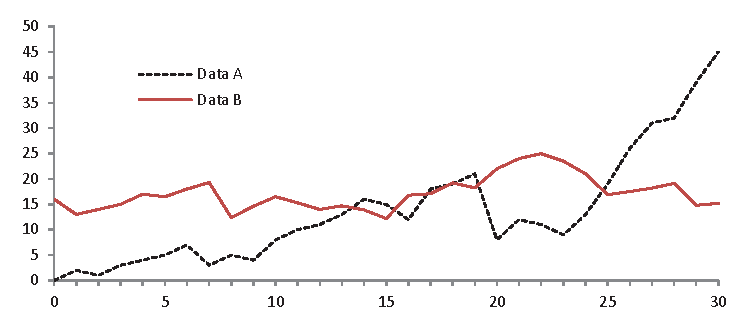
\includegraphics[width=\figscale\textwidth,center]{img/fig1.eps}
  \caption
  { 
  %\newline
    \textbf{A visual explanation.} You should be able to read the paper with just figures.
  }
  \label{fig:teaser}
\end{teaserfigure}

\maketitle
%\begin{figure}[h]
  \centering
  \vspace{-0.2cm}
  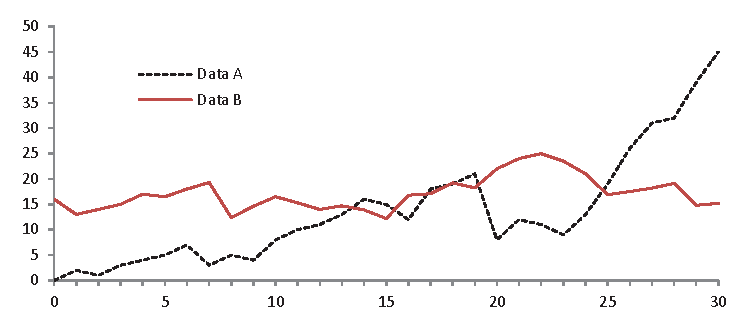
\includegraphics[width=\linewidth]{img/fig1.eps}
  \caption
  { 
  %\newline
    \textbf{A visual explanation.} You should be able to read the paper with just figures.
  }
  \label{fig:overview}
\end{figure} % Visual abstract
\begin{teaserfigure}
  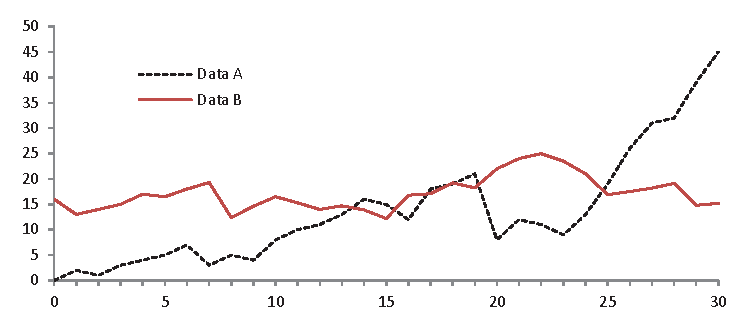
\includegraphics[width=\figscale\textwidth,center]{img/fig1.eps}
  \caption
  { 
  %\newline
    \textbf{A visual explanation.} You should be able to read the paper with just figures.
  }
  \label{fig:teaser}
\end{teaserfigure} % Visual abstract
\section{Introduction}
    \lipsum[1-6]

\section{Background}
	\subsection{Section 2.1}\label{sec:back1}	
	    MAP-Elites\cite{mapelites, me_nature}, QD\cite{pugh_qd, cully_qd}, Generative Designs\cite{bradner2014parameters, nagy2017beyond}.
\lipsum[1-2]

	\subsection{Section 2.2}\label{sec:back2}	
        \lipsum[1-2]
	
\section{Method}
	\subsection{The First Part}\label{sec:method1}	
	    \begin{figure*}[h]
  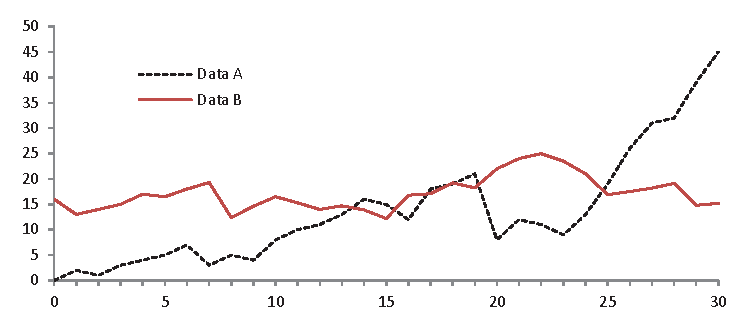
\includegraphics[width=\figscale\textwidth,center]{img/fig1.eps}
  \caption
  { 
  %\newline
    \textbf{A visual explanation.} You should be able to read the paper with just figures.
  }
  \label{fig:fig2}
\end{figure*}
\lipsum[1-3]
	\subsection{The Second}\label{sec:method2}	
        \begin{figure*}[ht]
  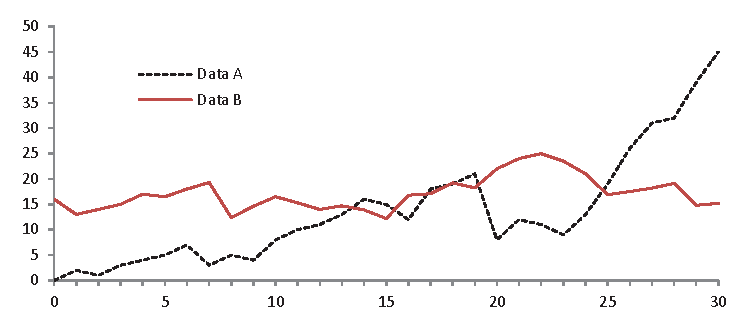
\includegraphics[width=\figscale\textwidth,center]{img/fig1.eps}
  \caption
  { 
  %\newline
    \textbf{A visual explanation.} You should be able to read the paper with just figures.
  }
  \label{fig:fig3}
\end{figure*}
\lipsum[1-3]
        
\section{Benchmark}
	\subsection{Setup}\label{sec:bench1}	
	    \lipsum[1-3]
	\subsection{Results}\label{sec:bench2}	
        \begin{figure*}[ht]
  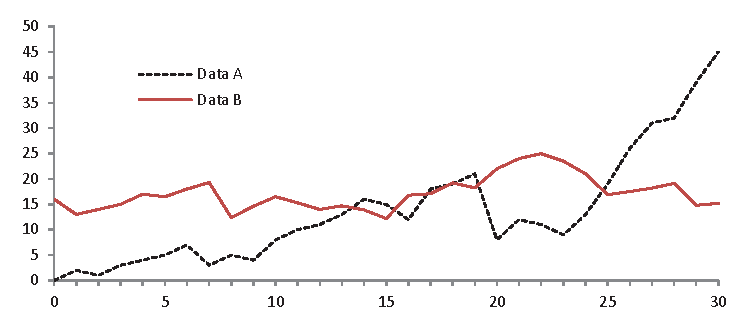
\includegraphics[width=\figscale\textwidth,center]{img/fig1.eps}
  \caption
  { 
  %\newline
    \textbf{A visual explanation.} You should be able to read the paper with just figures.
  }
  \label{fig:fig4}
\end{figure*}
\lipsum[1-3]

\section{Application}
	\subsection{Setup}\label{sec:app1}	
	    \lipsum[1-4]
	\subsection{Results}\label{sec:app2}	
        
\begin{figure*}[ht]
  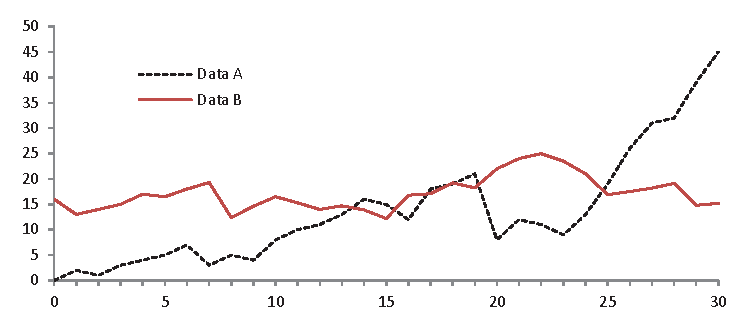
\includegraphics[width=\figscale\textwidth,center]{img/fig1.eps}
  \caption
  { 
  %\newline
    \textbf{A visual explanation.} You should be able to read the paper with just figures.
  }
  \label{fig:fig5}
\end{figure*}
\lipsum[1-3]
        
\section{Discussion}
        \lipsum[1-3]        
\bibliographystyle{template/ACM-Reference-Format}
\bibliography{bib/qd,bib/ml,bib/gd}
\newpage
\section{Supplemental Material}
Upon publication all supplemental material, along with all source code used to produce the results in this paper will be published online.

\end{document}
\endinput
%%
%% End of file `sample-sigconf.tex'.
